\documentclass[../../main.tex]{subfiles}
\begin{document}

\subsection*{8.11}
Un conduttore cilindrico cavo di raggi a e b è percorso da una corrente distribuita uniformemente.\\
Calcolare il campo magnetico B(r) in funzione della distanza $r$ dall'asse.\\
Ricavare i risultati relativi ad un conduttore cilindrico pieno.\\
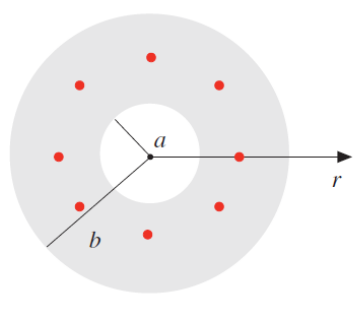
\includegraphics[scale=0.3]{e_8_11_0.png}\\
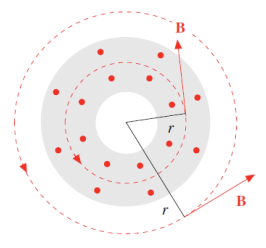
\includegraphics[scale=0.3]{e_8_11_1.png}
\subsubsection*{Formule utilizzate}
\subsubsection*{Soluzione punto a}
Dato che questa è una simmetria cilindrica posso semplificare la formula di Ampere.\\
$B(r) 2\pi r = \mu_0 i_{conc}$\\
se $r < a$: $B(r) = 0$\\
se $a < r < b$: $B(r) 2\pi r = \mu_0 i_{conc}$ con $i_{conc} = \frac{\pi \left(r^2 - a^2\right)}{\pi\left(b^2-a^2\right)}i$\\
se $r > b$: $B(r) = \frac{\mu_0 i}{2\pi r}$
\subsubsection*{Soluzione punto b}
Naso del cilindro pieno: ovvero quando a = 0. Posso utilizzare le funzioni trovate precedentemente con a = 0.
\newpage

\end{document}